\documentclass[runningheads]{llncs}
\usepackage[T1]{fontenc}
\usepackage{graphicx}
\usepackage{booktabs}
\usepackage{amsmath}
\usepackage{amssymb}
\usepackage{hyperref}
\usepackage{xcolor}
\hypersetup{colorlinks=true,linkcolor=black,citecolor=black,urlcolor=blue}

\begin{document}

\title{When Is a User's Own History Enough? A Controlled Study of
Peer-Isolated Personal Recommendation}

\author{Bidit Das}
\titlerunning{When Is a User's Own History Enough?}
\authorrunning{B. Das}
\institute{Independent Researcher, Plano, TX, USA\\
\email{biditdas18@gmail.com}}

\maketitle

\begin{abstract}
Personal data analytics systems often cannot consult other users: the data may be
on-device, legally siloed, or simply absent for a new deployment. We ask when
recommendation built \emph{exclusively} from a single user's own interaction history is
sufficient, and when it is not. We use Essence---a deliberately minimal peer-isolated
system pairing a frozen sentence encoder with per-user $K$-means and cosine
retrieval---as an instrument rather than a proposal, evaluating it against nine baselines
on three datasets spanning music, e-commerce and film.
Two findings emerge. First, the answer is governed by the density of cross-user
co-occurrence in the evaluated population, not by the content domain. Peer-isolated
retrieval ranks second and third of ten where that density is low (Last.fm-1K, Amazon
Books) and eighth of ten where it is high (MovieLens-25M); the pattern belongs to the
whole no-pooling architecture family rather than to any particular component. We
demonstrate the mechanism \emph{within a single dataset}: raising Last.fm-1K's user cap
lifts the share of items heard by two or more users from 10.3\% to 28.4\% and reverses the
verdict, from $d = +0.28$ in favour of peer-isolated retrieval over item-based
collaborative filtering to $d = -0.16$ against it, both significant. A domain is therefore
not weak or strong in collaborative signal; a \emph{cohort} is. Second, and centrally, the interest-clustering step contributes nothing
measurable. In the targeted test on the users whose taste is most clearly multi-modal it is
significant in none of 18 silhouette-stratified comparisons; and across the fourteen
dataset-level comparisons spanning three datasets, two sentence encoders, two user-activity
cohorts and two temporal-split protocols, exactly one favours clustering and one favours
simple recency-weighting, both marginal.
We report the single exception rather than suppress it, and show it falls below its own
detection threshold. We also report a two-sided bootstrap defect, present in our earlier
work, that counted tied resamples as evidence against the null and inflated significance
on sparse long-tail metrics. Baselines throughout are given the benefit of the doubt, a
convention that costs us one previously significant result.
\keywords{Personal data analytics \and Recommender systems \and Negative results
\and Cold start \and Reproducibility}
\end{abstract}

\section{Introduction}

A recommender that may not look at other users is an unusual object. Almost all deployed
systems pool behaviour across a population, and the dominant methods---collaborative
filtering, matrix factorisation, sequential models---are defined by that pooling. Yet a
growing class of settings forbids it. On-device assistants hold data that never leaves the
phone. Regulated domains silo records by subject. A new product has no population to pool
over. In each case the practical question is the same: \emph{how much is lost by modelling
a user from their own history alone?}

This paper answers that question empirically and reports a negative result at its
centre.\footnote{An earlier and substantially weaker version of this study appeared as a
non-archival poster at the New In ML workshop, NeurIPS 2026. References to ``our earlier
work'' throughout denote that version. The present paper supersedes it: the $K$-selection
rule, the significance testing, the baseline configurations and the headline finding itself
have all changed, and we document each change and the direction it moves our claims. Of the
analyses reported here, the encoder replication, the heavy-user and expanded-cohort
replications, the power analysis, the sequential baselines, the study-wide multiplicity
correction, the seed-stability check and the cohort-density result are new.}

We build a minimal peer-isolated system, Essence, and treat it as an instrument. Essence
embeds items with a frozen sentence encoder, partitions each user's history into $K$
interest clusters with $K$-means, selects the cluster nearest the user's recent activity,
and retrieves by cosine similarity. No component is novel and none is intended to be; the
system exists to isolate the variable of interest, which is the absence of cross-user
information.

\paragraph{Contributions.}
\begin{enumerate}
\item \textbf{A population-density result.} Peer-isolated retrieval is competitive where
cross-user co-occurrence is sparse and far behind where it is dense. We identify the
mediator by manipulating it \emph{within} a dataset --- twice, by two different means ---
rather than inferring it from a three-dataset contrast, and show the effect belongs to the
no-pooling family rather than to clustering.
\item \textbf{A clustering null, established at scope.} Per-user interest clustering gives
no measurable benefit over recency-weighted retrieval across three datasets, two encoders,
two activity cohorts and two split protocols, with a minimum detectable effect for every
comparison so the claim is bounded rather than asserted.
\item \textbf{A statistical correction.} We fix a tie-handling defect in the two-sided
bootstrap $p$-value used in our earlier work, which reported some zero-versus-zero
comparisons as maximally significant.
\item \textbf{Conservative reporting.} Baselines are reported at the better of their
published and validation-tuned configurations, costing us one previously significant
result.
\end{enumerate}

\section{Related Work}

\paragraph{Multi-interest recommendation.} MIND~\cite{li2019mind} and
ComiRec~\cite{cen2020controllable} represent each user by several interest vectors rather
than one, on the premise that a single embedding cannot capture heterogeneous taste. Both
learn those interests from pooled interaction data. Essence adopts the multi-interest
premise but removes the pooling, which is precisely what lets us ask whether the premise
survives in isolation.

\paragraph{Sequential recommendation.} GRU4Rec~\cite{hidasi2016session} and
SASRec~\cite{kang2018self} model the order of interactions. They require many users'
sequences to learn transition structure, and we include both as library implementations.

\paragraph{Content-based and cold-start methods.} Content-only retrieval avoids the
cold-start problem structurally by not requiring co-occurrence. This is a generic property
of the approach rather than a property of any particular system, a distinction the
literature does not always preserve and one we are careful to make.

\paragraph{Negative and reproducibility results.} Several authors have found that carefully
tuned simple baselines match or exceed neural recommenders~\cite{dacrema2019really,rendle2020neural}.
Our clustering null is of that kind, with the difference that the method whose component we
find inert is our own.

\section{Method}

Let user $u$ have interaction history $H_u = (i_1,\dots,i_n)$ in chronological order. Each
item $i$ carries text $t_i$ (title, artist or author, genre or category, description). We
embed with a frozen sentence encoder $\phi$, so $v_i = \phi(t_i)/\lVert\phi(t_i)\rVert$.
No interaction data enters $\phi$.

\paragraph{Interest clusters.} We run $K$-means on $\{v_i : i \in H_u\}$ to obtain
centroids $c_1,\dots,c_K$ for that user alone. If $|H_u| < K$ the user cannot be clustered
and falls back to the mean-embedding method; we report the frequency of this.

\paragraph{Active cluster and retrieval.} Let $r_u$ be the mean of the last ten items'
embeddings. We select $c^\star = \arg\min_k \lVert c_k - r_u \rVert$ and return the ten
unseen catalogue items of highest cosine similarity to $c^\star$.

\paragraph{Selecting $K$.} Our earlier work selected $K$ with a stopping rule evaluated
forward from a checkpoint at $K=8$, which a reviewer correctly identified as anchoring.
We replace it with a criterion that is anchoring-free by construction: choose the $K$
maximising validation Recall@10 subject to (a) mean items per cluster $\geq 3$ and
(b) every user clusterable. Constraint (a) prevents degenerate singleton clusters;
(b) prevents a configuration whose apparent quality is partly produced by fallback.
Table~\ref{tab:k} gives the outcome.

\begin{table}[t]
\caption{Adopted $K$ under the anchoring-free criterion. Both changes are forced by
constraints the original rule did not enforce.}\label{tab:k}
\centering
\small
\begin{tabular}{@{}lccp{5.1cm}@{}}
\toprule
Dataset & Published $K$ & Adopted $K$ & Reason for change \\
\midrule
Last.fm-1K & 10 & 10 & unchanged \\
Amazon Books & 10 & \textbf{8} & $K=10$ gives 2.58 items per cluster, below the floor of 3 \\
MovieLens-25M & 15 & \textbf{10} & at $K=15$ only ${\sim}90\%$ of users could cluster \\
\bottomrule
\end{tabular}
\end{table}

\begin{figure}[t]
\centering
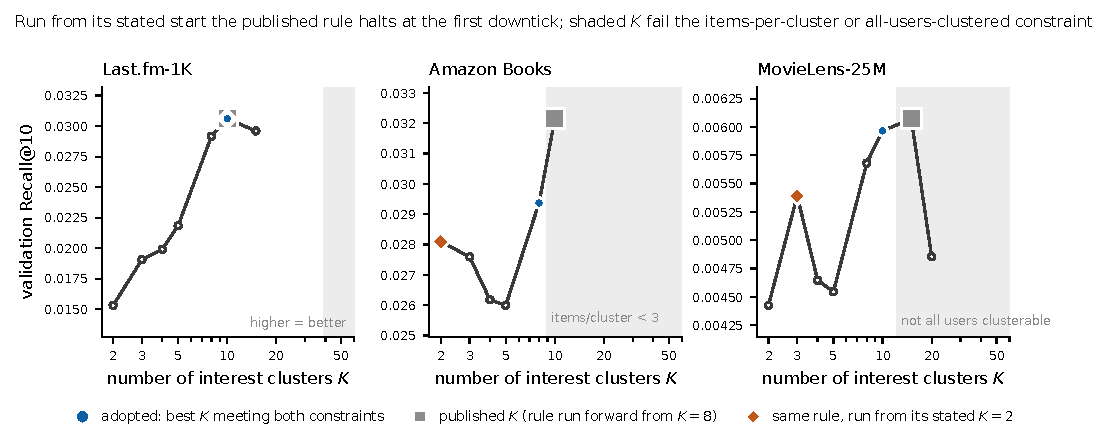
\includegraphics[width=0.92\textwidth]{fig_k_selection.pdf}
\caption{Validation Recall@10 against $K$ for each dataset, with grid points excluded by the
occupancy floor or the coverage constraint marked. The adopted $K$ is the constrained
maximiser, not the unconstrained one: on Amazon Books and MovieLens-25M the unconstrained
argmax violates a constraint the original rule did not enforce.}\label{fig:k}
\end{figure}

The adopted values are invariant to the sentence encoder. They are not, however, a property
of the domain: on Amazon Books the same criterion selects $K=8$ for users with ${\sim}29$
interactions and $K=60$ for users with 330 (Sect.~\ref{sec:heavy}). Any single reported $K$
is contingent on the user filter.

\section{Experimental Setup}

\paragraph{Datasets.} Three domains, chosen to span a range of collaborative signal
strength: music (Last.fm-1K), book retail (Amazon Books) and film (MovieLens-25M).
Users are filtered to an activity band and, for the two larger sets, sampled; this
gives 99, 2{,}000 and 2{,}000 users. Each history is split chronologically at that
user's own 80th percentile. We also report a global-cutoff variant
(Sect.~\ref{sec:leak}).

\paragraph{Baselines.} Nine: Recency-Weighted, Last-Item, Avg-Last-10, Content
(mean embedding), CF-ItemKNN, MIND, ComiRec, Popularity and Random, plus SASRec and
GRU4Rec as library-implemented sequential models (Sect.~\ref{sec:seq}).
Recency-Weighted is the critical one: it is Essence with the clustering step deleted, so
the Essence--Recency-Weighted contrast isolates clustering exactly.

\paragraph{Conservative baseline convention.} Each baseline is reported at the
\emph{better of its published and validation-tuned configuration on test}. This is
deliberately not the textbook protocol. We adopt it because strict validation-selection
would in one case have reported a ComiRec configuration 15.8\% worse on test than one we
had already run, turning a tuning artifact into an apparent win for our own system. The
convention favours the baselines and can only weaken our results. It costs us one
previously significant comparison, reported in Sect.~\ref{sec:domain}.

\paragraph{Statistics.} Paired bootstrap over users, 10{,}000 resamples, two-sided
$p$ counting exact ties in both tails, Benjamini--Hochberg FDR within family, Cohen's $d$
for paired differences. For every null we also report the minimum detectable effect at
80\% power, estimated from the bootstrap standard error (Sect.~\ref{sec:power}).

\section{Results}

\subsection{Domain dependence}\label{sec:domain}

\begin{table}[t]
\caption{Recall@10 at adopted $K$. Baselines at the better of published and tuned.
Best per dataset in bold.}\label{tab:main}
\centering
\small
\begin{tabular}{@{}lccc@{}}
\toprule
System & Last.fm-1K & Amazon Books & MovieLens-25M \\
\midrule
\textbf{Essence} & 0.0281 & 0.0246 & 0.0055 \\
Recency-Weighted & \textbf{0.0304} & 0.0260 & 0.0076 \\
Last-Item & 0.0265 & \textbf{0.0311} & 0.0091 \\
Avg-Last-10 & 0.0252 & 0.0235 & 0.0064 \\
Content (Avg Emb) & 0.0038 & 0.0173 & 0.0043 \\
CF (ItemKNN) & 0.0018 & 0.0031 & \textbf{0.0850} \\
MIND & 0.0082 & 0.0072 & 0.0423 \\
ComiRec (SA) & 0.0243 & 0.0056 & 0.0706 \\
Popularity & 0.0023 & 0.0021 & 0.0517 \\
Random & 0.0001 & 0.0001 & 0.0012 \\
\bottomrule
\end{tabular}
\end{table}

Table~\ref{tab:main} shows the pattern: Essence ranks second and third of ten on
Last.fm-1K and Amazon Books, and eighth of ten on MovieLens-25M, where CF-ItemKNN alone
beats it by more than an order of magnitude. Table~\ref{tab:metrics} shows the ordering
survives every cutoff and NDCG@10.

\begin{table}[t]
\caption{Essence holds the same rank under every metric on both datasets where the full
set was computed; MIND and ComiRec are re-scored from the same ranked lists. Two
disclosures, neither changing any ordering: the Amazon ComiRec row uses its tuned
configuration, 16\% below the conservative value in Table~\ref{tab:main}, and the
MovieLens rows are re-runs at $\mathrm{lr}=10^{-3}$, $K=4$, within $-0.8\%$ and $+11.2\%$
of published.}\label{tab:metrics}
\centering
\small
\begin{tabular}{@{}lcccccc@{}}
\toprule
& \multicolumn{3}{c}{Amazon Books} & \multicolumn{3}{c}{MovieLens-25M} \\
\cmidrule(lr){2-4}\cmidrule(lr){5-7}
System & R@5 & R@10 & NDCG@10 & R@5 & R@10 & NDCG@10 \\
\midrule
Last-Item & 0.0238 & 0.0311 & 0.0364 & 0.0076 & 0.0091 & 0.0151 \\
Recency-Weighted & 0.0170 & 0.0260 & 0.0273 & 0.0044 & 0.0076 & 0.0111 \\
\textbf{Essence} & 0.0162 & 0.0246 & 0.0262 & 0.0035 & 0.0055 & 0.0078 \\
Avg-Last-10 & 0.0154 & 0.0235 & 0.0243 & 0.0042 & 0.0064 & 0.0101 \\
Content (Avg Emb) & 0.0111 & 0.0173 & 0.0174 & 0.0019 & 0.0043 & 0.0052 \\
MIND & 0.0043 & 0.0072 & 0.0071 & 0.0248 & 0.0470 & 0.0546 \\
ComiRec (SA) & 0.0027 & 0.0047 & 0.0043 & 0.0399 & 0.0700 & 0.0899 \\
CF (ItemKNN) & 0.0019 & 0.0031 & 0.0032 & 0.0469 & 0.0850 & 0.1093 \\
Popularity & 0.0014 & 0.0021 & 0.0021 & 0.0307 & 0.0517 & 0.0712 \\
Random & 0.0000 & 0.0001 & 0.0001 & 0.0009 & 0.0012 & 0.0021 \\
\bottomrule
\end{tabular}
\end{table}

The effect is not a property of clustering. Recency-Weighted---identical to Essence but
with no clustering at all---exhibits the same profile, ranking first on Last.fm-1K and
collapsing on MovieLens-25M. What the data separate is architectures that pool across users
from architectures that do not.

\paragraph{What the conservative convention costs.} Essence significantly outperforms
MIND on both sparse datasets and ComiRec on Amazon Books, but is \emph{indistinguishable
from a properly tuned ComiRec on Last.fm-1K} ($d=0.065$, $q=0.54$): tuning closed that gap
from $2.05\times$ to $1.15\times$, and our earlier claim rested on a ComiRec denied a fair
learning rate. The comparison is also underpowered (detectable effect 0.0159 against an
observed 0.0038), so the two are \emph{not shown to differ} at $n=99$---not equal. The
defensible claim is thus narrower than before: peer-isolated retrieval is \emph{competitive
with} tuned multi-interest recommenders where co-occurrence is sparse, and far behind where
it is dense.

\subsection{The clustering null}\label{sec:null}

\begin{figure}[t]
\centering
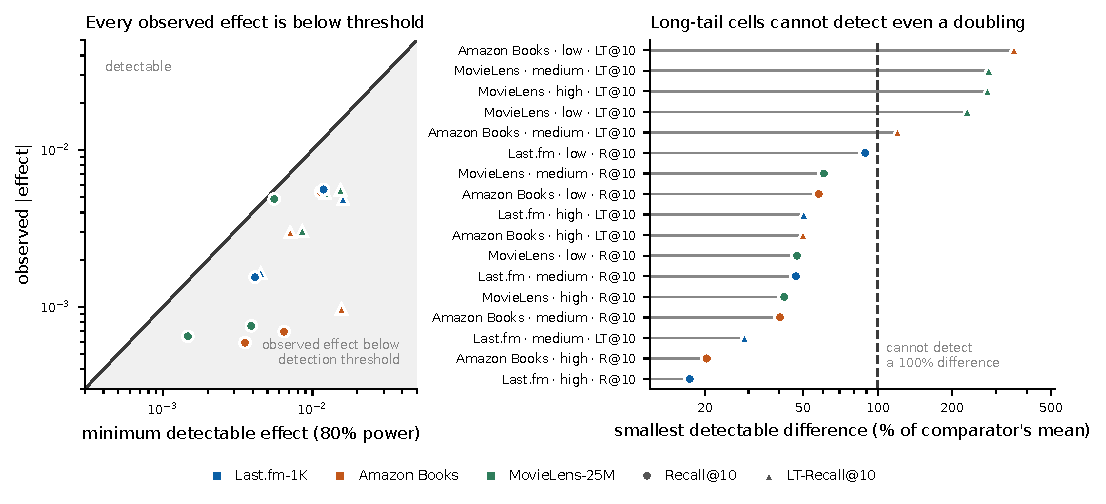
\includegraphics[width=0.78\textwidth]{fig_power.pdf}
\caption{Observed effect against minimum detectable effect at 80\% power for every null
comparison. Points below the diagonal are effects the test could not have detected.
Ranking-metric nulls are adequately powered; several long-tail cells are not and are
not claimed.}\label{fig:power}
\end{figure}

The sharpest version of the test restricts attention to the users whose taste is most
clearly multi-modal, stratifying by silhouette score: if clustering helps anyone, it should
help them. At validation-selected $K$, with tie-aware $p$ and no rows excluded, clustering
is significant in none of those 18 stratified comparisons against recency-weighted
retrieval. Our earlier work reported ``one of sixteen'', where the sixteen were a
hand-curated subset---formed, we later found, by dropping exactly the degenerate cases the
defect in Sect.~\ref{sec:bug} produced---and the one significant row was itself an artifact
of that defect.

Table~\ref{tab:robust} states the null at full scope.

\begin{table}[t]
\caption{Every Essence versus Recency-Weighted comparison in this study.}\label{tab:robust}
\centering
\small
\begin{tabular}{@{}llp{4.0cm}@{}}
\toprule
Robustness check & Configuration & Null holds? \\
\midrule
Main analysis & 3 datasets, adopted $K$ & yes \\
Second sentence encoder & all-mpnet-base-v2, 2 datasets & yes (0 of 8 favour clustering) \\
Heavy users & 330 interactions/user, $K=60$ & yes ($q=0.31$, powered to 21.6\%) \\
Global temporal cutoff & single wall-clock split & Recall@10 yes; \textbf{one exception} \\
Silhouette-stratified & most multi-modal users & yes \\
\bottomrule
\end{tabular}
\end{table}

Across all fourteen comparisons---three datasets, two encoders, two activity cohorts, two
split protocols---exactly one favours clustering and one favours recency-weighting, both
marginal.

\paragraph{The exception, reported and not claimed.} Under the global cutoff, clustering
beats recency-weighting on long-tail recall at $q=0.0496$. It is not an artifact of
fallback users: restricted to the 357 users who genuinely cluster, it survives at
$p=0.0348$, $d=0.096$. We nonetheless decline to claim it. The observed effect is
$0.64\times$ its own 80\%-power detection threshold, placing it in the regime where
significant findings are most inflated; it is one comparison out of fourteen, where 0.7
false positives are expected at $\alpha=0.05$; and $d=0.09$ is negligible beside the
effects the rest of the paper turns on.

\subsection{Statistical power}\label{sec:power}

A null is only informative if the test could have detected an effect. Of 18 null
comparisons, 17 are informative and none reach their own minimum detectable
effect (Fig.~\ref{fig:power}). The comparisons split cleanly into two regimes. Nulls on
ranking metrics are adequately powered and carry content. Several long-tail cells cannot
detect even a doubling of the comparator, and we do not assert those as nulls---a
correction to our earlier work, which did.

\subsection{Heavy users}\label{sec:heavy}

All three datasets bound user activity from above, which raises an obvious objection: the
excluded heavy users are the most plausibly multi-modal, so the clustering null may have
been established on the population least likely to exhibit the effect it tests.

We replicated on Amazon Books users with 201--1000 interactions (1{,}757 users, 330
interactions each against ${\sim}29$, catalogue 213{,}221 items, identical text coverage),
re-selecting $K=60$ for that cohort so clustering received its best configuration. The null
holds: Recall@10 difference $-0.000288$ ($d=-0.027$, $q=0.31$) with the test powered to
detect a 21.6\% relative difference. Clustering does not help the users it was supposed to
help.

Two secondary observations. Essence slips from third to fourth of the eight comparable
systems, and CF-ItemKNN degrades by only 22\% where content methods lose 86--93\%: heavy
users supply the co-occurrence signal CF needs. This is the mechanism of
Sect.~\ref{sec:cohort} appearing a second time, in a different dataset and under a
different manipulation --- raising the activity floor rather than lifting the ceiling ---
and it is the reason we frame the first finding as population density rather than domain.

\subsection{Encoder sensitivity}

Replacing all-MiniLM-L6-v2 (384-dim) with all-mpnet-base-v2 (768-dim) leaves conclusions
intact. Essence improves slightly (Amazon Books 0.0246 to 0.0254, rank three to two) and
only one of eighteen significance verdicts changes. Selected $K$ is identical under both
encoders. As a correctness check, the five systems that do not consume item
embeddings return bit-identical results while exactly the five that do consume them move.

\subsection{Sequential baselines}\label{sec:seq}

SASRec and GRU4Rec were run through RecBole with learning rates tuned on held-out
validation, and scored with our own metric implementations from the library's ranked lists.
Both fail on these datasets: Essence leads by $20.9\times$ and $23.3\times$ on Last.fm-1K
and by $174.6\times$ and $59.3\times$ on Amazon Books. Even taking each model's
best test configuration---a deliberately unfair comparison that favours the
baselines---the gap is $11.9\times$ to $43.6\times$.

The cause is structural rather than a tuning failure. Amazon Books is 0.063\% dense with 32
training items per user, so there is very little transition structure to learn. This is the
same weak-collaborative-signal condition our thesis concerns, and the result is therefore
consistent with it rather than incidental. It is emphatically \emph{not} evidence that
Essence outperforms SASRec in general; on denser data we would expect the ordering to
reverse, as it already does for the other collaborative baselines on MovieLens-25M.

\subsection{Temporal leakage}\label{sec:leak}

Per-user chronological splitting allows one user's training window to overlap another's
test window, which can favour collaborative methods. Under a single global cutoff every
system degrades, but unevenly: CF-ItemKNN loses 86\% where content and recency methods lose
37--45\%, and Essence's rank improves from third to second of eight. The leakage was
inflating the collaborative baselines, so our main protocol is the conservative choice for
this paper's central comparison.

\subsection{Is the domain difference real? A formal test}\label{sec:interaction}

Ranks describe the pattern; they do not test it. We therefore test the interaction directly.
For each collaborative baseline we compute the paired effect size (Cohen's $d$) of Essence
against it within each dataset, bootstrap each dataset's $d$ independently (10{,}000
resamples), and take the distribution of the difference. $d$ is scale-free, which matters
because absolute recall differs by an order of magnitude across these datasets.

\begin{table}[t]
\caption{The between-dataset difference as an interaction, not a ranking. $\Delta d$ is the
change in Essence's effect size when moving from a sparse-co-occurrence dataset to
MovieLens-25M. Every contrast is significant after BH correction and every one is a sign
flip: Essence ahead becomes Essence behind. These hold for the datasets \emph{as
configured}; Sect.~\ref{sec:cohort} shows Last.fm-1K's position is set by its user cap, not
by its domain.}\label{tab:interaction}
\centering
\small
\begin{tabular}{@{}llcccc@{}}
\toprule
Baseline & Sparse-density set & $d$ (weak) & $d$ (MovieLens) & $\Delta d$ & 95\% CI \\
\midrule
CF (ItemKNN) & Last.fm-1K & $+0.28$ & $-0.55$ & 0.83 & [0.76, 0.95] \\
CF (ItemKNN) & Amazon Books & $+0.25$ & $-0.55$ & 0.80 & [0.76, 0.84] \\
MIND & Last.fm-1K & $+0.24$ & $-0.38$ & 0.62 & [0.54, 0.76] \\
MIND & Amazon Books & $+0.21$ & $-0.38$ & 0.58 & [0.54, 0.63] \\
ComiRec (SA) & Last.fm-1K & $+0.07$ & $-0.52$ & 0.58 & [0.33, 0.72] \\
ComiRec (SA) & Amazon Books & $+0.22$ & $-0.52$ & 0.74 & [0.70, 0.78] \\
Popularity & Last.fm-1K & $+0.27$ & $-0.44$ & 0.71 & [0.63, 0.82] \\
Popularity & Amazon Books & $+0.26$ & $-0.44$ & 0.69 & [0.65, 0.74] \\
\bottomrule
\end{tabular}
\end{table}

All 8 contrasts are significant after BH correction, all 8 show a sign flip, and no
confidence interval contains zero; the smallest lower bound is 0.33. $\Delta d$ ranges
from 0.58 to 0.83, which are large effects. The difference between datasets is therefore a
tested claim rather than a described pattern. Sect.~\ref{sec:cohort} then shows that a
dataset's position on this axis is set by its cohort rather than its domain: Last.fm-1K's
$d$ against CF-ItemKNN changes sign when its user cap is lifted, so the contrasts above
hold for these datasets \emph{as configured} and should not be read as properties of
music, book retail or film.

\subsection{Cohort density, not domain, drives the verdict}\label{sec:cohort}

Sect.~\ref{sec:interaction} establishes that Essence's standing differs between datasets.
It does not establish \emph{why}, and the natural reading --- that music and book retail
simply carry weaker collaborative signal than film --- turns out to be wrong. The Last.fm-1K
cohort is capped at 500 distinct tracks per user, which admits 99 of the 975 users clearing
the minimum. Lifting that cap to 2{,}000 admits 374, and reverses the result.

\begin{table}[t]
\caption{The same dataset, the same domain, the same code and seed. Raising the user cap
raises cross-user co-occurrence and reverses the verdict against item-based collaborative
filtering. Mean training history rises from 215 to 783 items per user and the candidate
catalogue from 18{,}679 to 158{,}074 items, so absolute recall falls for every system;
only within-row comparisons are meaningful.}\label{tab:cohort}
\centering
\small
\begin{tabular}{@{}lccccc@{}}
\toprule
Cohort (tracks/user) & Users & Items w/ $\geq 2$ users & Essence & CF-ItemKNN & $d$ \\
\midrule
50--500 (published) & 99 & \textbf{10.3\%} & 0.0281 & 0.0018 & $\mathbf{+0.28}$ \\
50--2{,}000 & 374 & \textbf{28.4\%} & 0.0026 & 0.0055 & $\mathbf{-0.16}$ \\
\bottomrule
\end{tabular}
\end{table}

Both verdicts are significant ($q < 0.0001$ and $q = 0.014$). On the expanded cohort
CF-ItemKNN is the best of the eight systems and Essence falls from second to fifth. The
mediating quantity is in the fifth column: item-based collaborative filtering requires
cross-user co-occurrence, and the expanded cohort supplies nearly three times as much of it.

This reframes the first finding rather than overturning it. Signal strength is a property
of the \emph{evaluated population}, not the content domain, and the three-dataset pattern
is three points on that one axis --- which is why MovieLens-25M, the densest, is where
peer-isolated retrieval fails worst. It is also actionable: measure co-occurrence density
in your own user base rather than reason from your product category.

\paragraph{A confound we cannot remove.} Lifting the cap raises the user count (99 to 374)
and the history length (215 to 783 items/user) together. Both raise density, so both act
through the same mediator, but this design cannot separate them: isolating user count would
need 374 users with 50--500 interactions and only 99 exist. We claim density as the
mediator, not which of its causes dominates. MIND and ComiRec are omitted from
Table~\ref{tab:cohort}: trained on the 99-user sample, they cover only 26.5\% of the
expanded cohort, and mixing a 99-user evaluation into a 374-user ranking is the error this
paper elsewhere reports catching. The clustering null is unaffected and moves marginally
further against clustering (LT-Recall@10 $q = 0.031$).

\subsection{Study-wide multiplicity}\label{sec:multi}

FDR above is controlled within each family, which is conventional but invites a fair
question: how many hypotheses does this study test in total? The answer is 136. Applying
Benjamini--Hochberg across all 136 at once takes the significant count from 59 to 56 and
changes exactly two rows, both against clustering.

First, the one exception in Sect.~\ref{sec:leak} --- the single comparison in this study where
clustering beat recency-weighting --- is not significant study-wide ($q = 0.075$). We had
already declined to claim it on power grounds; the stricter correction independently agrees.
Under it, \emph{no comparison anywhere in this study shows clustering significantly
outperforming recency-weighted retrieval}.

Second, one comparison becomes significant that was not: in the silhouette-stratified test the
\emph{high}-silhouette stratum --- the users whose histories separate most cleanly into
distinct interest groups, which is precisely the population the multi-interest premise
concerns --- shows clustering performing significantly \emph{worse} than recency-weighting
($q = 0.033$). This is not a paradox: BH adapts to the distribution of $p$-values it is given, and a
family of 18 mostly-null tests is a less favourable reference than the full study. It is the strongest form the negative result takes. On the
users where interest clustering should help most, it measurably hurts.

We report within-family FDR as the primary correction and state the study-wide result
alongside it. Reporting only the former would preserve an exception we do not believe;
reporting only the latter would overstate the certainty of a post-hoc choice.

\subsection{Seed stability}\label{sec:seeds}

Two seeds were fixed and never varied: the per-user $K$-means initialisation and the random
user sample. Both were re-run on Amazon Books at the adopted $K$. The clustering null holds in
all five configurations, and significance counts are identical across the three clustering
seeds and across the two user samples; no verdict depends on either seed.

Worth stating explicitly, since the opposite would be a fair criticism: the published seed is
mildly \emph{unfavourable} to Essence. At \texttt{random\_state=42} the comparison against
Recency-Weighted gives $q = 0.52$; the two alternative seeds give $q = 0.61$ and
$q = 0.90$, i.e.\ further from significance, and Essence scores 8.0\% higher under them
on average. The published configuration does not flatter the method.

\subsection{The identity shortcut, at the adopted \texorpdfstring{$K$}{K}}\label{sec:shortcut}

Our earlier work reported that roughly 20\% of Essence's hits share an artist with the user's
active cluster, and that excluding same-artist candidates collapses performance by 85--90\%.
That analysis was run at $K = 3$, a value this paper does not adopt --- an inconsistency we
found while re-verifying it. At $K = 3$ the figures reproduce exactly (20.6\% shortcut share,
87.9\% collapse). At the adopted $K = 10$ the dependence is substantially larger:
\textbf{32.9\% of hits are same-artist and removing those candidates costs 95.3\% of
performance}.

More clusters means tighter, more artist-homogeneous clusters, so nearest-centroid retrieval
lands closer to artists already inside the active cluster. The shortcut is a property of the
retrieval geometry and it grows with $K$. Restating it at the adopted $K$ therefore sharpens
rather than softens the limitation: a large part of what this architecture recovers is
identity matching, not taste modelling.

\paragraph{Cold start.}\label{sec:cold} At the adopted $K$, content-only retrieval beats CF-ItemKNN in 5 of
6 popularity-decile comparisons at the two coldest deciles across the three datasets, the
exception being MovieLens's second decile where CF has begun to acquire signal. This is a
generic consequence of not requiring co-occurrence, not a property of Essence, and it is the
same mechanism as Sect.~\ref{sec:cohort} at the item level rather than the population level.

\subsection{A statistical defect in our earlier work}\label{sec:bug}

The two-sided bootstrap $p$-value was computed as $\min(1, 2\min(f, 1-f))$ with
$f = \mathrm{mean}(\delta > 0)$ over resampled differences $\delta$. This counts every
resample with $\delta = 0$ as evidence against the null. On long-tail recall, where most
users score exactly zero, the resample distribution has large mass at zero, so a
one-sided-with-ties difference was reported as $p = 0$---including cases in which both arms
were identically zero for every user and no difference existed to detect.

We fixed this in all call sites by counting ties in both tails. The correction is
consequential and moves against us: the clustering-value test falls from seven of eighteen
significant to none of 18. We verified the fix is surgical rather than
wholesale---one dataset's corrected output is byte-identical to its published counterpart.

\section{Discussion and Conclusion}

The practical question has a conditional answer: a user's own history is enough when
cross-user co-occurrence is thin and not enough when it is dense. That boundary belongs to
the \emph{cohort}, not the domain --- the same music data sits on either side of it
depending on the user cap --- so the diagnostic for a practitioner under an on-device or
siloed-data constraint is not which algorithm to pick, but whether their user base supplies
dense co-occurrence.

The clustering null carries a narrower lesson. The multi-interest premise---that users hold
several tastes one vector cannot capture---may well be true; our data show only that
recovering them by unsupervised partition of one user's embedded history yields nothing a
recency-weighted query does not already have.

\paragraph{Conclusion.} Peer-isolated retrieval is a viable design where co-occurrence is
sparse and a poor one where it is dense, and that boundary is set by the cohort rather than
by the domain. Within the design, per-user interest clustering---the component we
originally proposed as the contribution---adds nothing measurable over simple recency
weighting across every robustness dimension we tested.

\paragraph{Limitations.} Item text quality bounds every content method here and we did not
vary it. The long-tail nulls are underpowered and we do not claim them. The main Last.fm-1K
analysis has 99 users, which limits power on that dataset; Sect.~\ref{sec:cohort} reports
the expanded cohort. Sequential baselines on Amazon Books use a split agreeing with ours on
92.8\% of test items rather than exactly.

\begin{thebibliography}{8}
\bibitem{li2019mind}
Li, C., et al.: Multi-interest network with dynamic routing for recommendation at Tmall.
In: CIKM, pp. 2615--2623 (2019)

\bibitem{cen2020controllable}
Cen, Y., Zhang, J., Zou, X., Zhou, C., Yang, H., Tang, J.: Controllable multi-interest
framework for recommendation. In: KDD, pp. 2942--2951 (2020)

\bibitem{hidasi2016session}
Hidasi, B., Karatzoglou, A., Baltrunas, L., Tikk, D.: Session-based recommendations with
recurrent neural networks. In: ICLR (2016)

\bibitem{kang2018self}
Kang, W.-C., McAuley, J.: Self-attentive sequential recommendation. In: ICDM,
pp. 197--206 (2018)

\bibitem{dacrema2019really}
Dacrema, M.F., Cremonesi, P., Jannach, D.: Are we really making much progress? A worrying
analysis of recent neural recommendation approaches. In: RecSys, pp. 101--109 (2019)

\bibitem{rendle2020neural}
Rendle, S., Krichene, W., Zhang, L., Anderson, J.: Neural collaborative filtering vs.
matrix factorization revisited. In: RecSys, pp. 240--248 (2020)

\bibitem{reimers2019sentence}
Reimers, N., Gurevych, I.: Sentence-BERT: sentence embeddings using Siamese BERT-networks.
In: EMNLP-IJCNLP, pp. 3982--3992 (2019)

\bibitem{zhao2021recbole}
Zhao, W.X., et al.: RecBole: towards a unified, comprehensive and efficient framework for
recommendation algorithms. In: CIKM, pp. 4653--4664 (2021)
\end{thebibliography}

\end{document}
